% !TEX TS-program = pdflatex
% !TEX encoding = UTF-8 Unicode

% This is a simple template for a LaTeX document using the "article" class.
% See "book", "report", "letter" for other types of document.

\documentclass[11pt]{article} % use larger type; default would be 10pt

\usepackage[utf8]{inputenc} % set input encoding (not needed with XeLaTeX)

%%% Examples of Article customizations
% These packages are optional, depending whether you want the features they provide.
% See the LaTeX Companion or other references for full information.

%%% PAGE DIMENSIONS
\usepackage{geometry} % to change the page dimensions
\geometry{a4paper} % or letterpaper (US) or a5paper or....
% \geometry{margin=2in} % for example, change the margins to 2 inches all round
% \geometry{landscape} % set up the page for landscape
%   read geometry.pdf for detailed page layout information

\usepackage{graphicx} % support the \includegraphics command and options

% \usepackage[parfill]{parskip} % Activate to begin paragraphs with an empty line rather than an indent

%%% PACKAGES
\usepackage{booktabs} % for much better looking tables
\usepackage{array} % for better arrays (eg matrices) in maths
\usepackage{paralist} % very flexible & customisable lists (eg. enumerate/itemize, etc.)
\usepackage{verbatim} % adds environment for commenting out blocks of text & for better verbatim
\usepackage{subfig} % make it possible to include more than one captioned figure/table in a single float
% These packages are all incorporated in the memoir class to one degree or another...

%%% HEADERS & FOOTERS
\usepackage{fancyhdr} % This should be set AFTER setting up the page geometry
\pagestyle{fancy} % options: empty , plain , fancy
\renewcommand{\headrulewidth}{0pt} % customise the layout...
\lhead{}\chead{}\rhead{}
\lfoot{}\cfoot{\thepage}\rfoot{}

%%% SECTION TITLE APPEARANCE
\usepackage{sectsty}
\allsectionsfont{\sffamily\mdseries\upshape} % (See the fntguide.pdf for font help)
% (This matches ConTeXt defaults)

%%% ToC (table of contents) APPEARANCE
\usepackage[nottoc,notlof,notlot]{tocbibind} % Put the bibliography in the ToC
\usepackage[titles,subfigure]{tocloft} % Alter the style of the Table of Contents
\renewcommand{\cftsecfont}{\rmfamily\mdseries\upshape}
\renewcommand{\cftsecpagefont}{\rmfamily\mdseries\upshape} % No bold!

%%% END Article customizations

%%% The "real" document content comes below...

\title{Project planning and current technical structure}
\author{Cees-Jan Nolen, Robert Kraaijeveld, Steven Schenk}
\date{28-9-16}

\begin{document}
  \pagenumbering{gobble}
  \maketitle
  \newpage
  \pagenumbering{arabic}
  \tableofcontents

\newpage
\section{Introduction}
This document will explain the current technical configuration and structure for our internship project concerning procedural avatar generation. 

~\\
A quick recap of what our project is aiming to achieve: We want to create a game for the Experience Room which contains procedurally generated avatars, with each avatar possessing a personality. The avatars should then perform certain actions or respond to situations according to its' personality. The player will be able to walk amongst the NPC population and will be presented various tasks, most of them revolving around recognizing which avatars exhibit which personality traits (For example: Select the avatar who you think is the most egoistic.).

~\\
The data resulting from these experiments could then be used for further study.


\newpage
\section{Reference}
In the below image you can see a complete diagram of our system, with each sub-system or algorithm displayed here having a reference to the chapter of this document in which it is discussed.

~\\
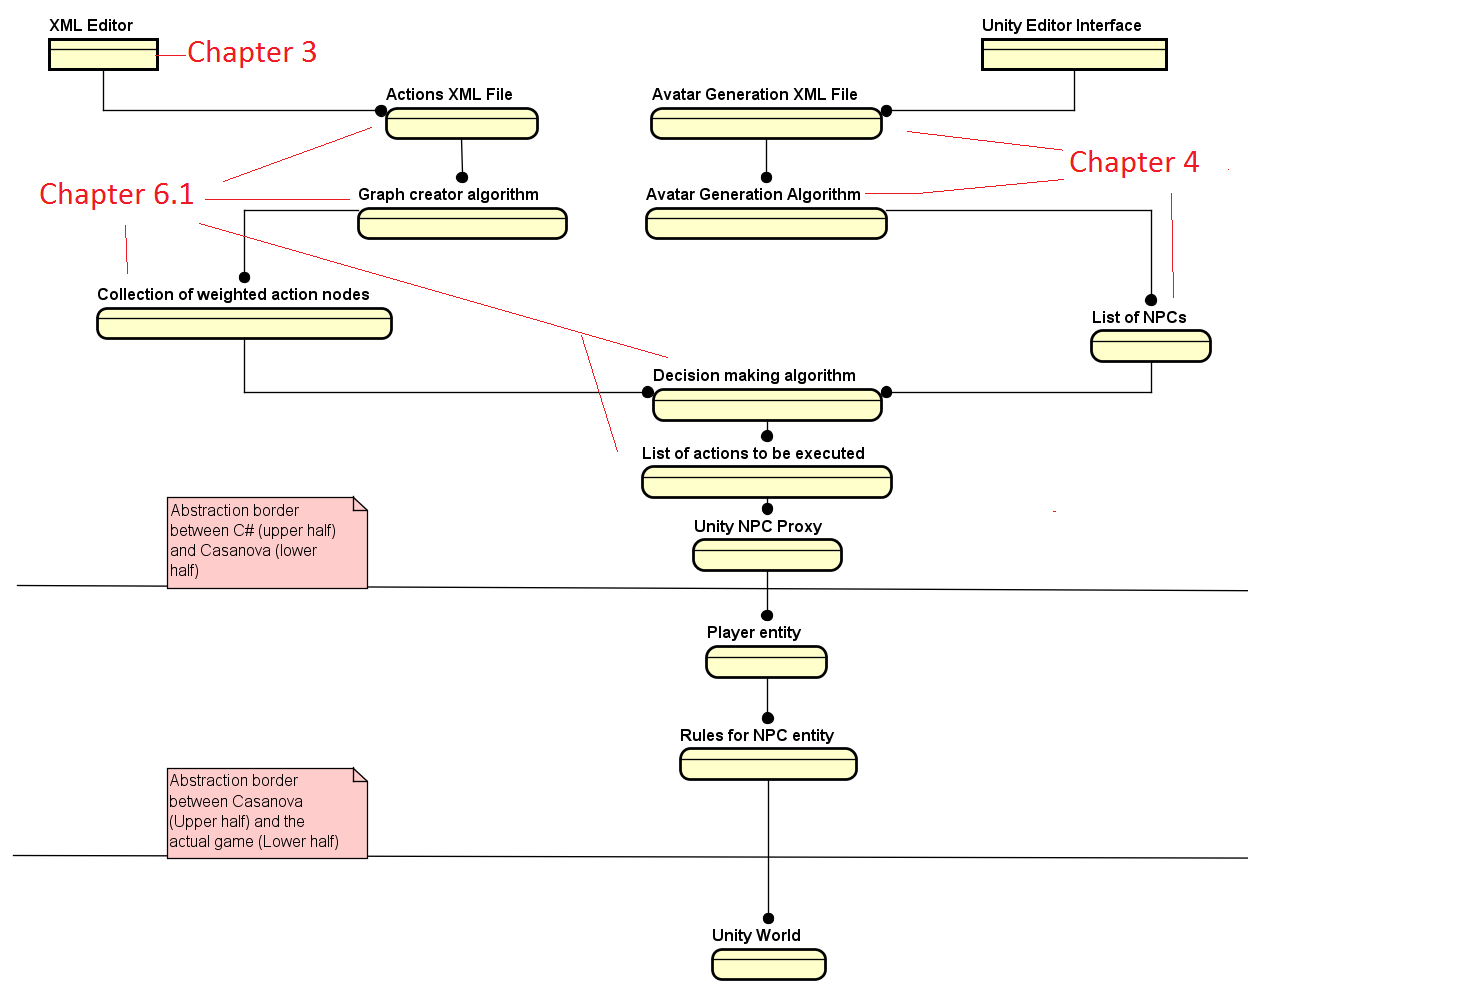
\includegraphics[width=20cm, height=13cm]{ReferenceEr}


\newpage
\section{Our frameworks and languages}
For this project, we are using a combination of Unity and the included C Sharp programming language, combined with the Casanova Programming Language. We use XML files to store settings such the possible actions that an NPC can take.
Casanova is a very high level language, capable of easily manipulating game states. It uses a proxy system, consisting of C Sharp classes, to import Unity GameObjects and the like without having to deal with the relatively low level Unity code. The below image gives a visual example of this system.


~\\
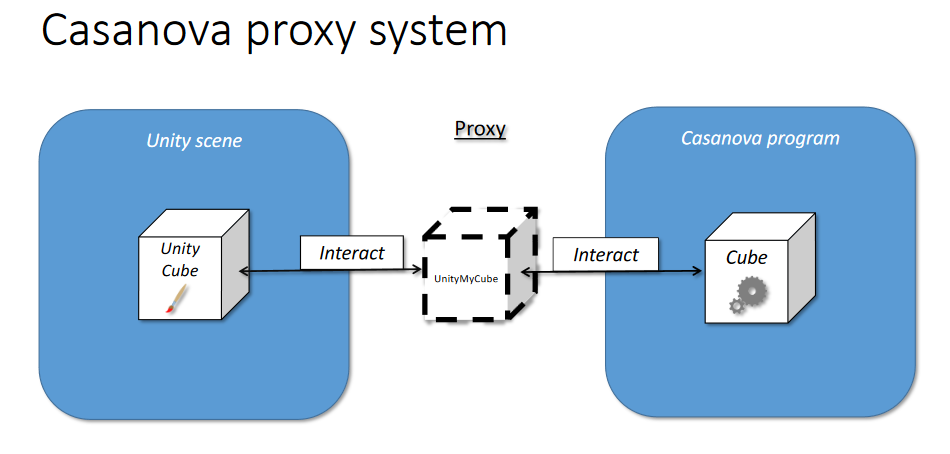
\includegraphics[scale=0.5]{proxySystem}
~\\

\newpage
\
As mentioned earlier, we use various XML files to store information or settings relative to our game. In order to make editing these files (specifically, the XML file which actions an NPC can take) easier, especially for non-programmers, we have created a simple GUI for editing these files, which runs locally in the users browser. 

~\\
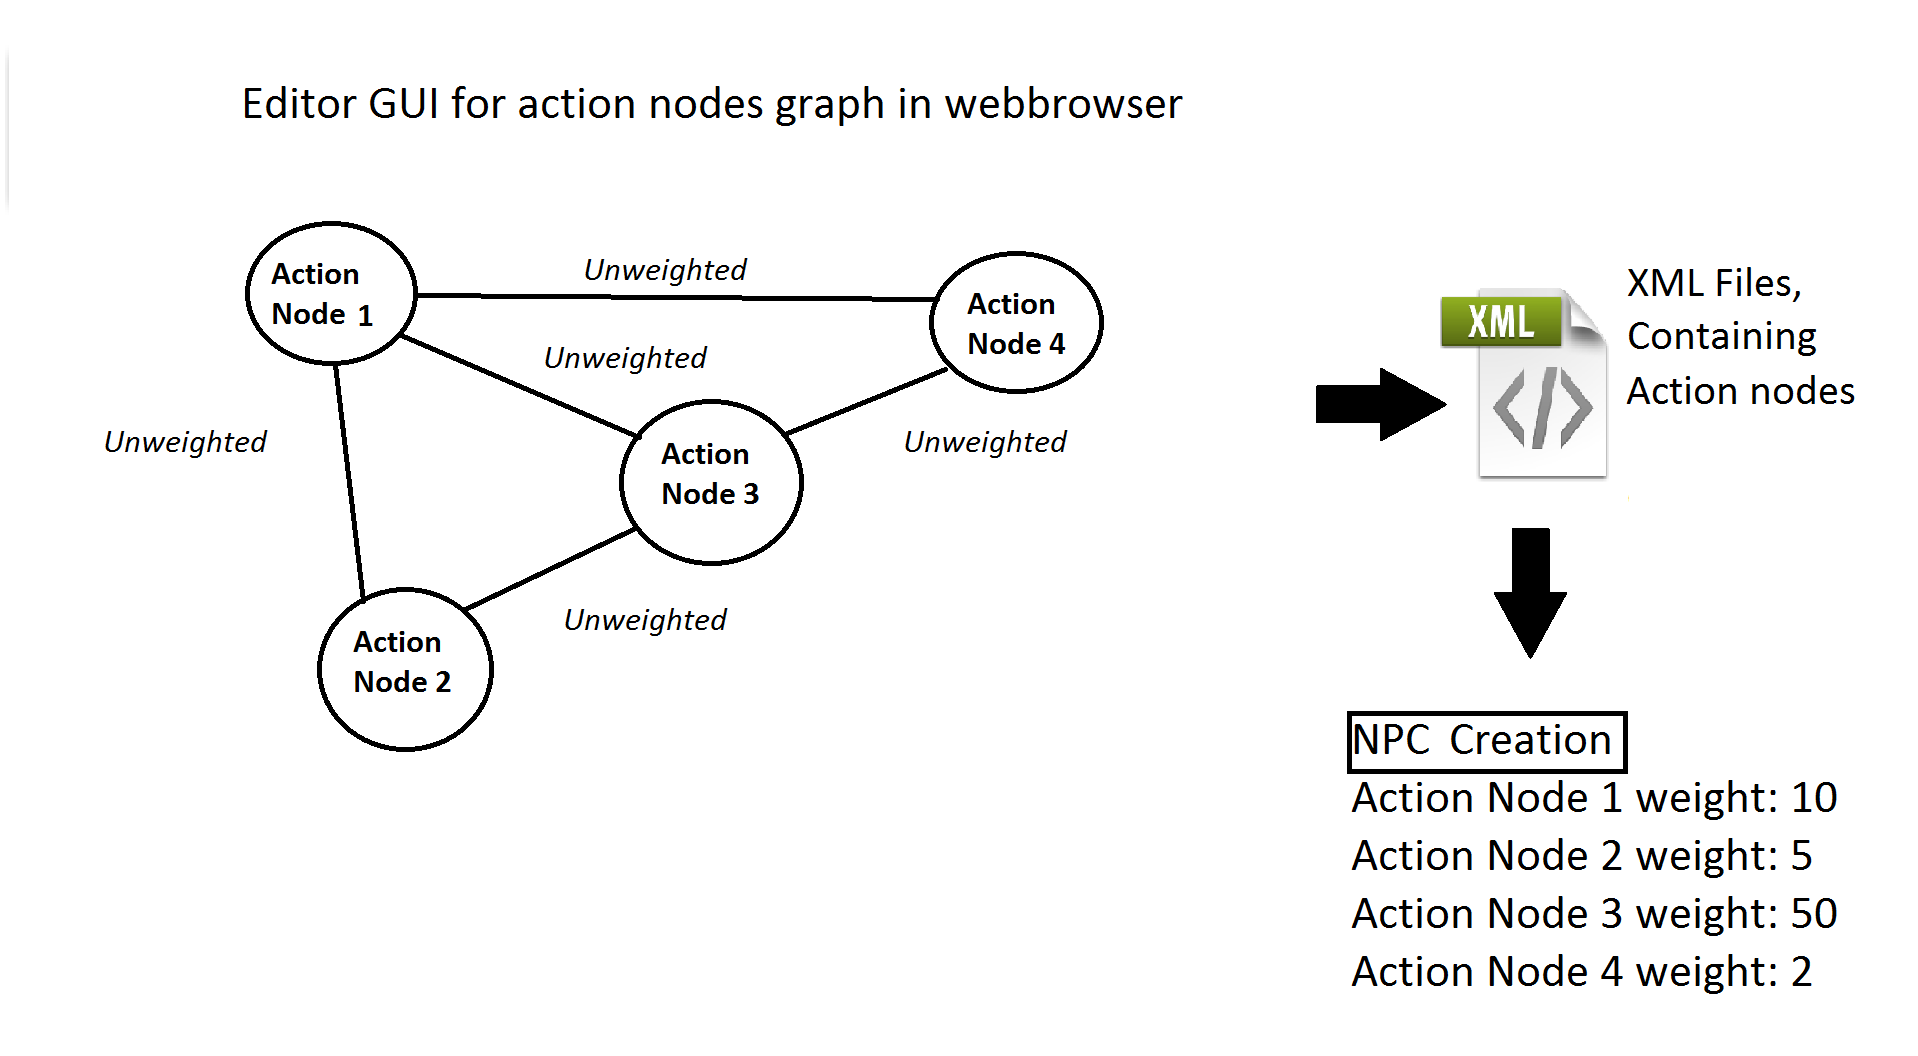
\includegraphics[scale=0.3]{XmlSystem}
~\\

~\\
We implemented this editor in Python, using the lightweight 'Bottle' framework.

\newpage
\section{Our personality model}
Currently, we are using primary factors 1-4 of the big 5 personality model to provide our NPC's with personality values. To recap, the primary factors of the big 5 personality model are as follows:

\begin{enumerate}
\item Agreeableness (Which we use under the name 'Egoism vs. Altruism')
\item Extraversion vs. Introversion
\item Thoroughness vs. Conscientiousness
\item Emotional Stability vs. Neuroticism
\end{enumerate}

~\\
The 5th factor is 'Openness to experience' which we found nearly impossible to implement as concrete game behavior: Therefore we have forfeited its use for now.

~\\
Note that when we model these values to an NPC, they receive 8 values instead of 4: One value for each extreme of the factors, with the values ranging from 0 up to and including 100.
For instance:

~\\
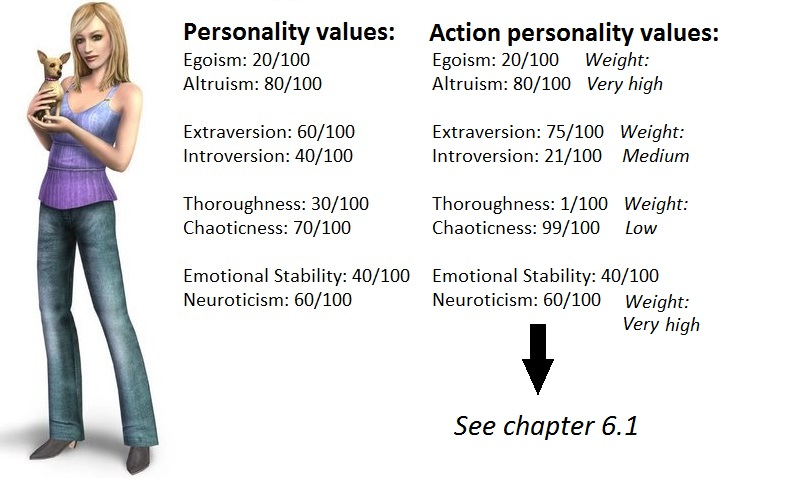
\includegraphics[scale=0.7]{sim}
~\\
The action nodes that we saw earlier are weighted differently for each NPC, because each NPC has different personality values. The algorithm we use to achieve this is discussed in chapter 6.1.

\newpage
\section{General System Structure}
The below ER Diagram documents the high level structure of our system:

%IMAGE
~\\
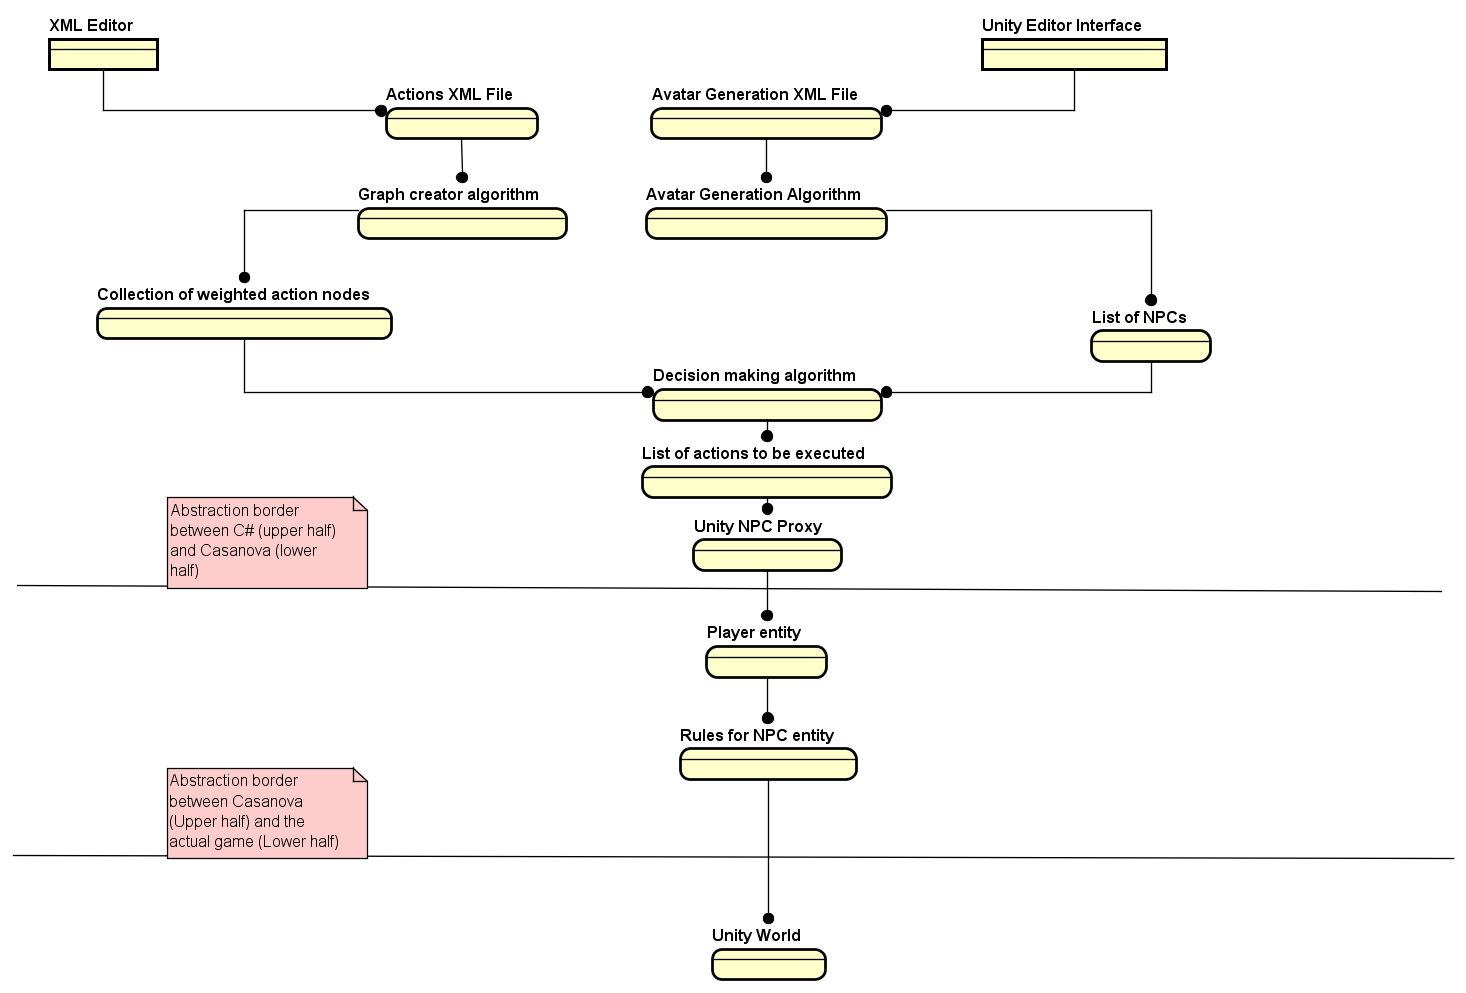
\includegraphics[width=20cm, height=13cm]{SystemEr}
~\\

\newpage
As you can see, the C Sharp code is mainly responsible for setting up the appropriate datastructures and algorithms enabling an NPC to make decisions based on its personality, whilst Casanova is only responsible for translating the resulting list of actions into actual in-game behavior. 

~\\
We decided to let Casanova handle most of the actual game-logic rather than create algorithms etc in it because Casanova is platform-independent: This enables our game logic to be directly imported into other game frameworks. 

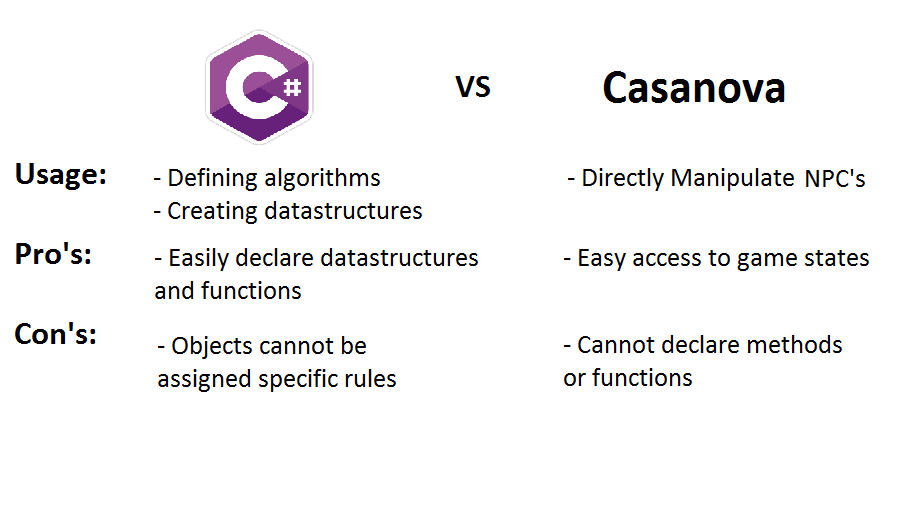
\includegraphics[scale=0.7]{CSHARPVSCASANOVA}

Contrary to C Sharp however, Casanova is not very usefull for creating large algorithms and datastructures: It has no mechanic for declaring functions or methods outside of game rules, and it only supports a very small number of datastructures natively. 

\newpage
\section{NPC behavior}
In our project, each NPC gets his own collection of personality factors and assorted values ranging from 0 to 100, like we talked about earlier. 

~\\
Finally, they have a collection of accumulated personality values, which use the same 8 factors as their earlier mentioned personality values. These accumulated values will come into play in the decision making algorithm. Initially, these accumulated values are all zero, but they are summed with the personality modifiers of each actions that the NPC chooses to take: This process will be explained in more detail later.

~\\
NPC's can display their personalities to the player in one of three ways:

~\\
Through actions that they decide to execute because these actions' personality values are proportionate to their own.

~\\
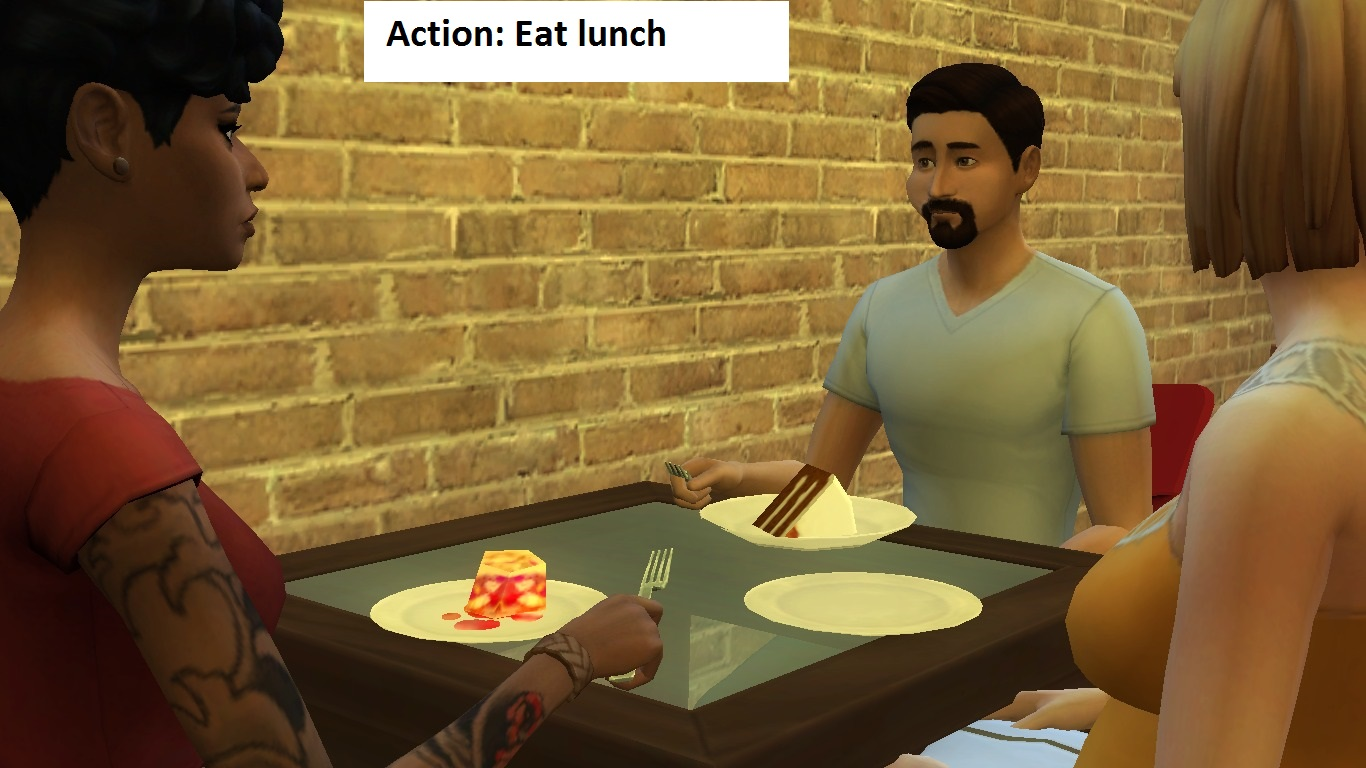
\includegraphics[scale=0.4]{SimsEating}


\newpage
We want to incorporate emotions into actions as well, making NPC's who are very sad execute their actions in, well, a very sad manner. How exactly we will implement this is still up for debate; see chapter 7 for more details.
~\\

~\\
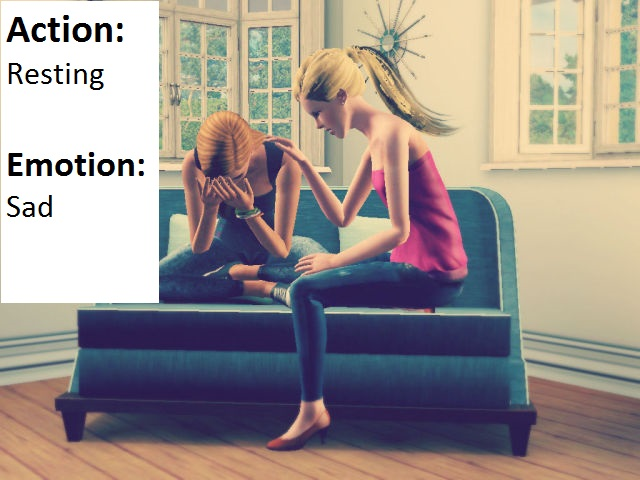
\includegraphics[scale=0.4]{SimsCrying}
~\\

Finally, NPC's can react to (and display their personalities) through events: occurences which can trigger an immediate reaction from the NPC.
~\\

~\\
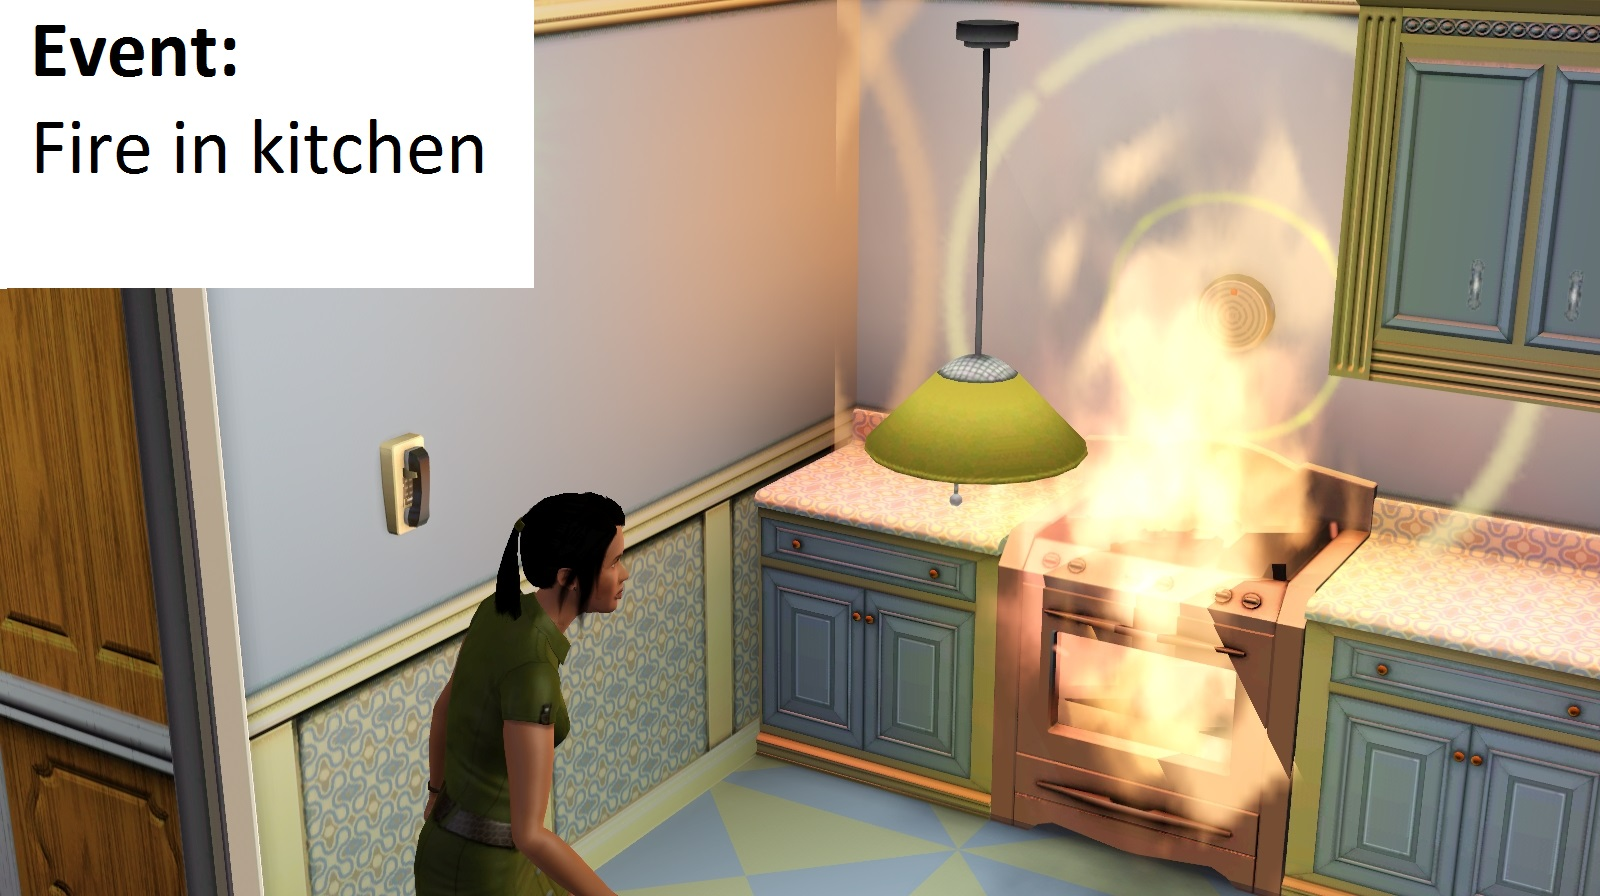
\includegraphics[scale=0.4]{SimsFire}
~\\

~\\
Up next, we will discuss each of these kinds of behavior in detail.

\newpage
\subsection{Actions and graph creation algorithm}
We define an XML file containing a list of actions. Each action has the following properties:

~\\
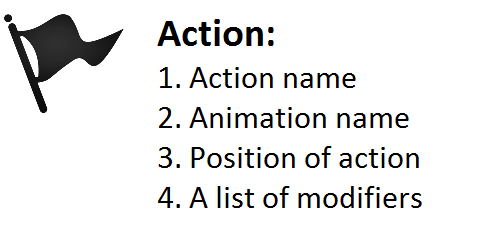
\includegraphics[scale=0.7]{ActionFlag}
~\\

~\\
The first three properties speak for themselves, but the fourth property deserves some more detailed explanation. The list of modifiers is a list consisting of the same 8 personality-extremes as an NPC possesses; These values are used later in the graph creation algorithm.

~\\
Now that we have defined a series of actions, we create an initial weighted, undirected graph as a datastructure for these actions. This graph does however not permit visiting the same node twice, since this could potentially result in an NPC constantly repeating the same action. 

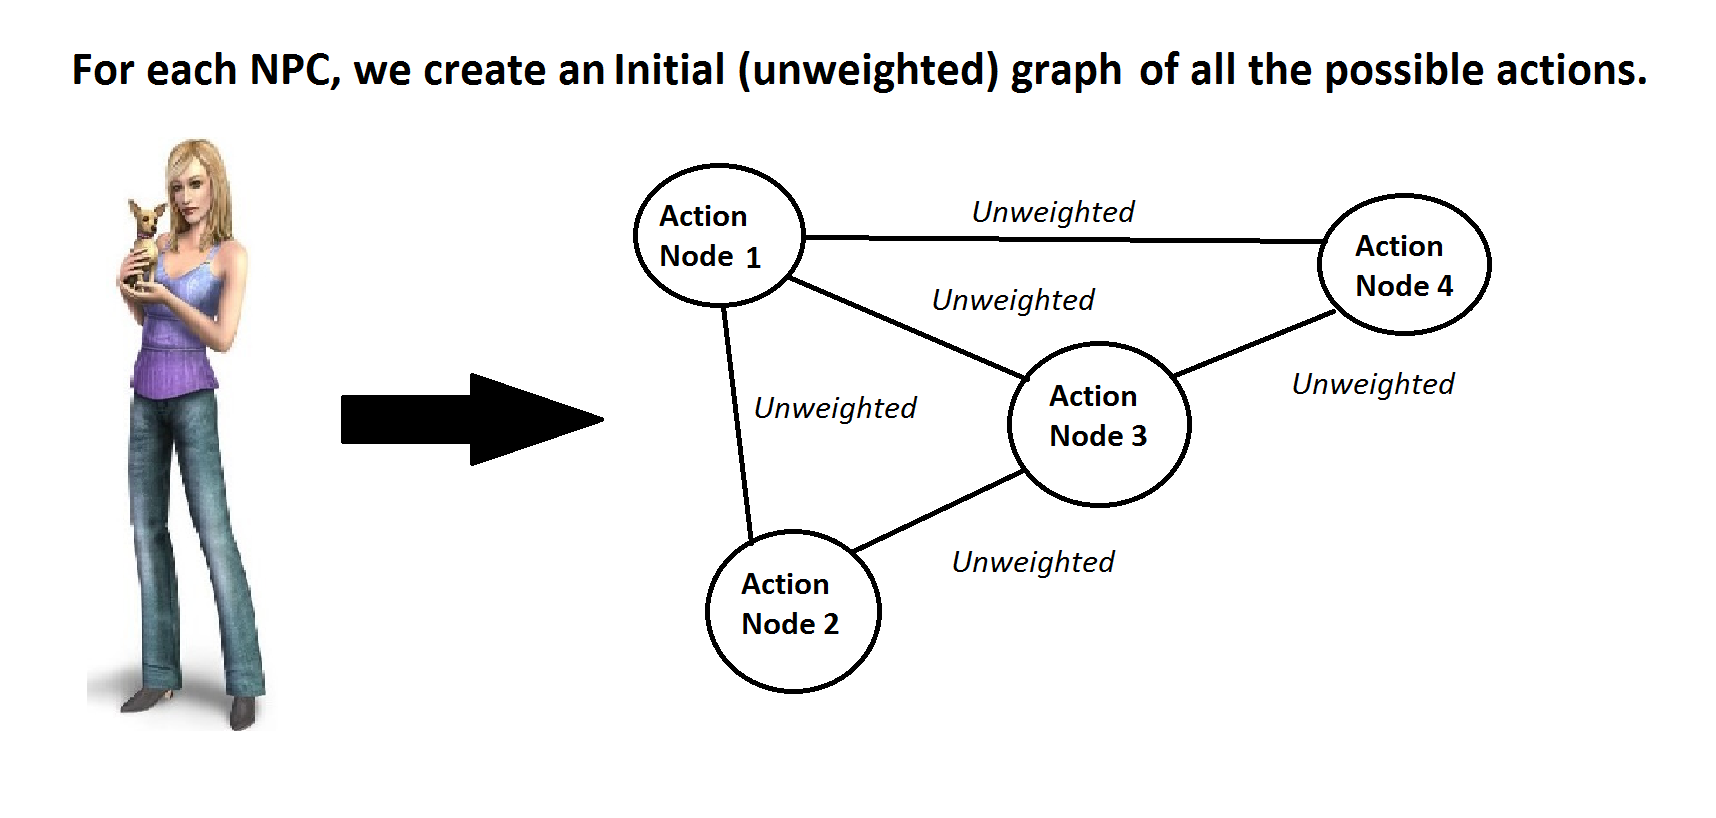
\includegraphics[scale=0.4]{InitialGraph}

~\\
Note that since every NPC has different personality values, they each get their own weighted graph of actions. 



\newpage
This is done by calculating the dot product between an action's modifier value and the appropriate personality value for the NPC. 

~\\
This process is repeated for each personality value of the NPC, producing a total weight for the given action. Done for each action, this algorithm produces a weighted graph of all the actions for a specific NPC.


~\\
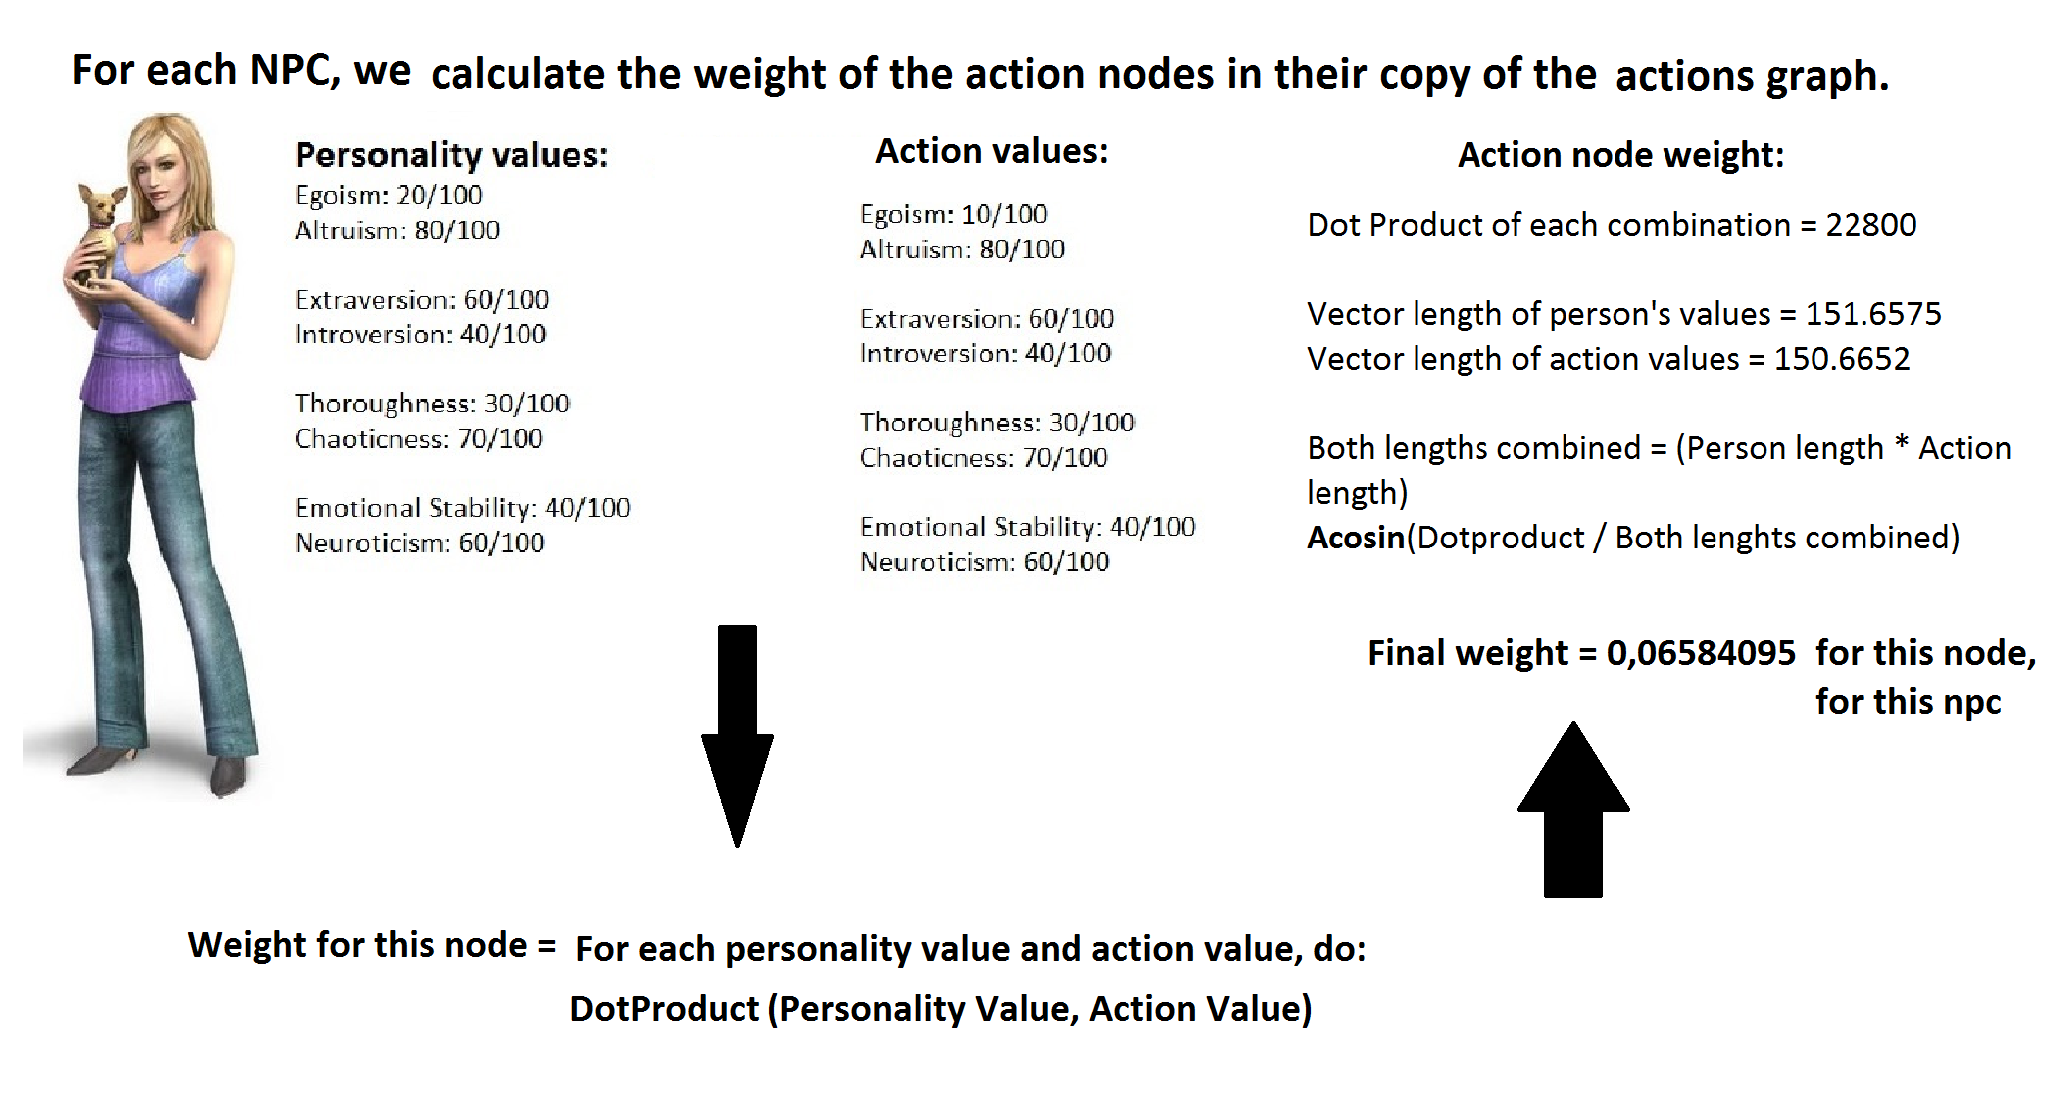
\includegraphics[scale=0.4]{FillingAlgorithm}


~\\
Very important to note is that this first weighted graph, and only this first graph, uses the fixed (!) personality values of the NPC: Further weighted graphs use the accumulated values which are modified by the actions that an NPC takes.



\newpage
After the initial graph has been created and the NPC is spawned in the gameworld, a random action node is selected as a starting node. The starting node is added to the list of actions which will be passed to Casanova, and the NPC's accumulated values are summed with the action's modifier values. 

~\\
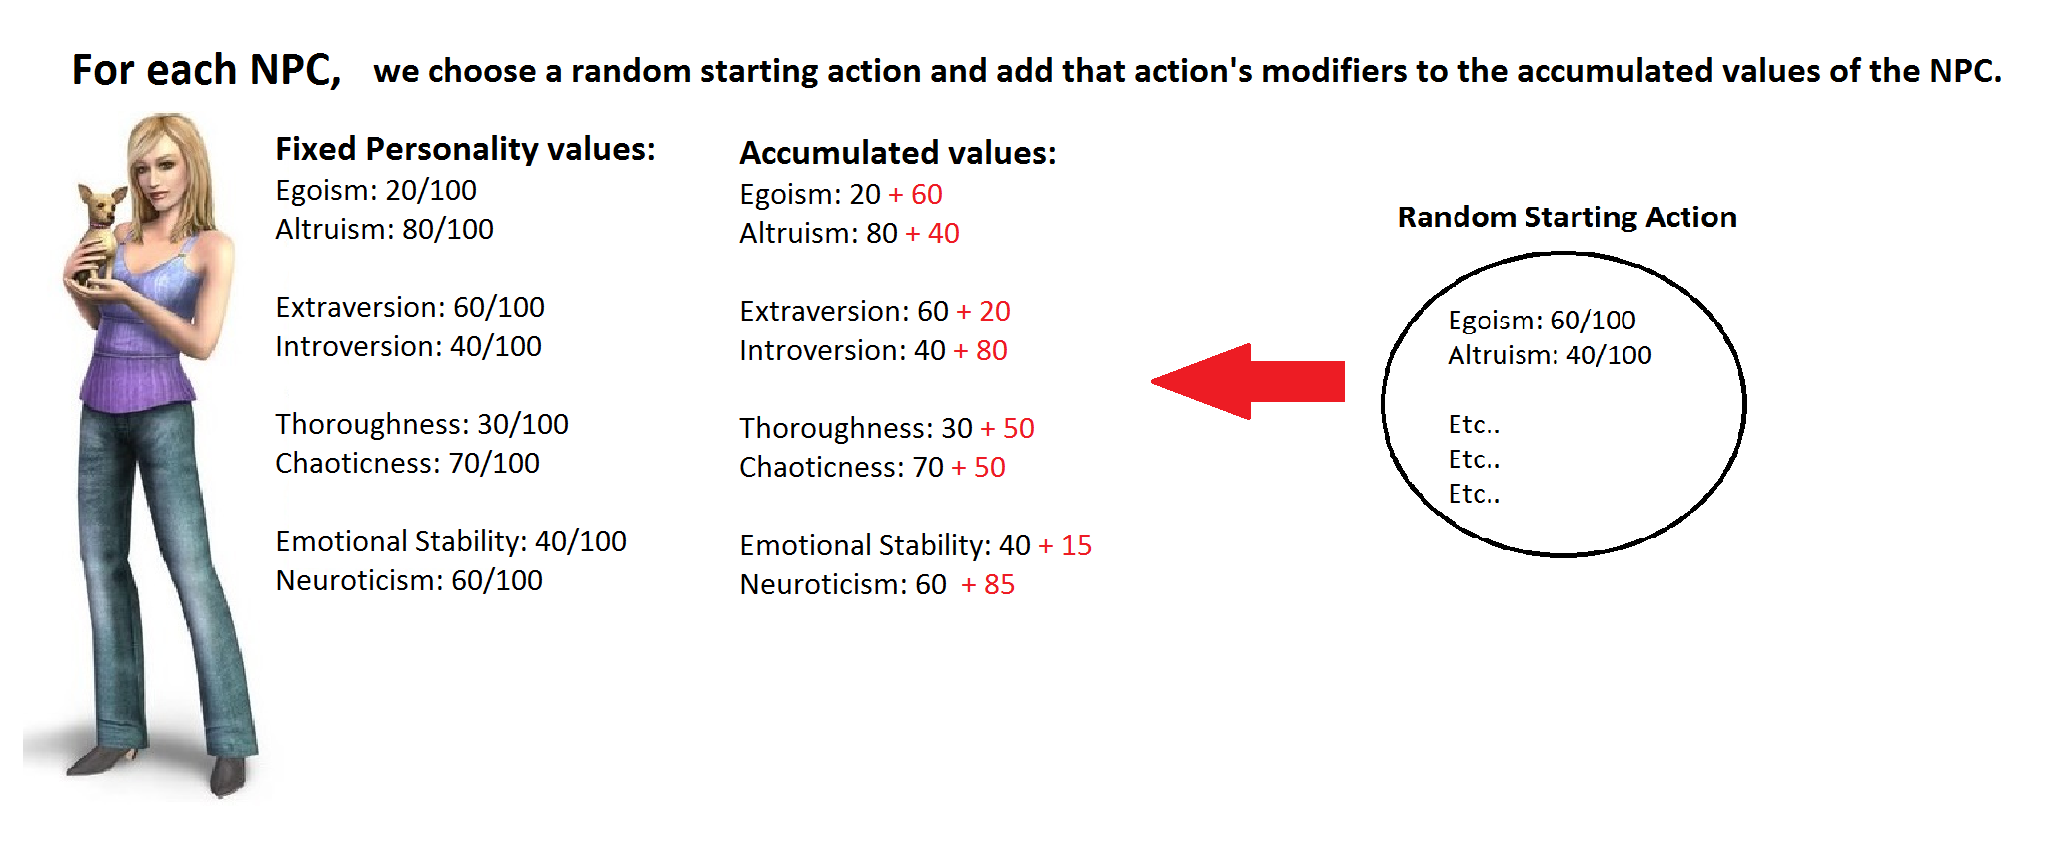
\includegraphics[width=17cm, height=7.5cm]{DecisionMakingAlgorithm}

~\\
After that, the decision making algorithm marks the current node as 'visited', chooses the neighbour of the current action with the highest weight, sets it to be the new current action and adds it to the list of actions. The process then starts again with the new current node as starting node. 

~\\
Note that given enough time, this algorithm will add each action in the graph to the list: The solution to this problem is described in the next page.



\newpage
Every 10 seconds of game-time Casanova requests a fresh list of actions from this algorithm. The Unity proxy responds to this request by re-creating the weighted graph, using the accumulated values from the previous actions instead of the fixed personality values of a NPC, like we mentioned earlier. This constant refreshing ensures two things: 

~\\
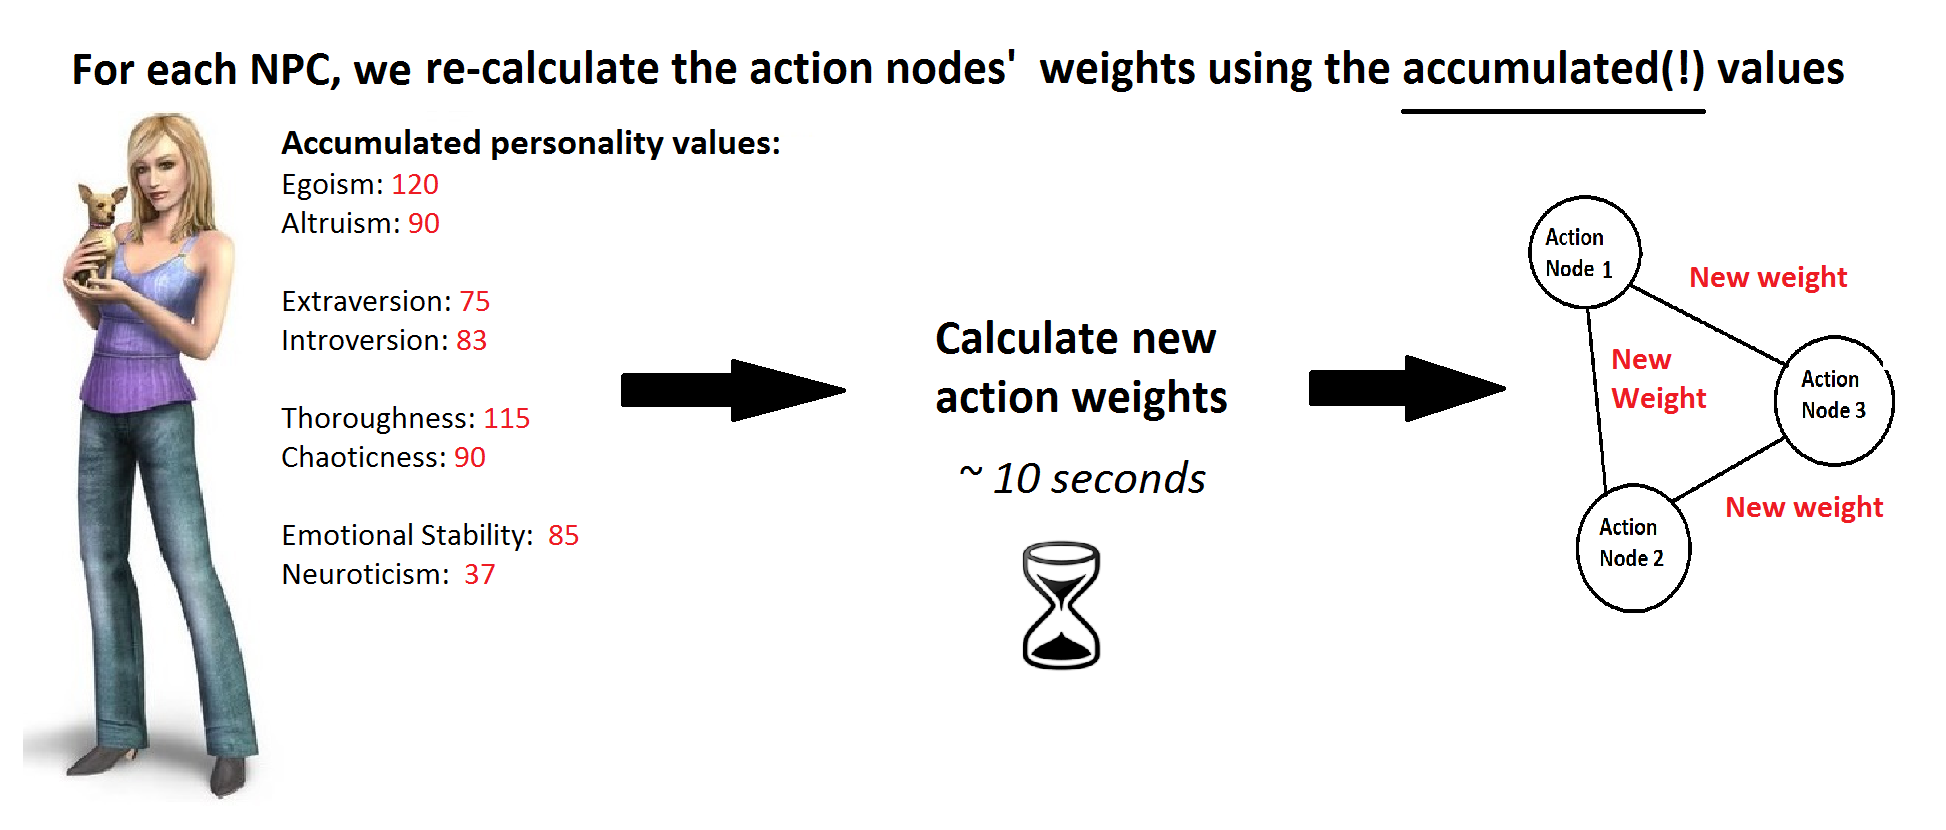
\includegraphics[width=17cm, height=7.5cm]{AccumulatedValues}

~\\
Firstly, that Casanova only executes the first few actions in the resulting actions list, so that the NPC does not execute each piece of behavior in the graph (Which is not desirable, since then it would be impossible to see what kind of personality a given NPC possesses.). 

~\\
Secondly, that an NPC's experiences changes his later behavior by way of his/hers accumulated values. 
The 10 second time-mark can of course be altered, and we are still experimenting with different time thresholds in order to create the most realistic behavior.

\newpage
\subsection{Improving this algorithm by using maximum weight matching}
The current algorithm produces relatively sensible NPC behavior, but only chooses one action at a time: There is no planning involved. We want to have our NPC's planning their actions in advance, because this more accurately mimics human behavior. 

~\\
To accomplish this, we will use a maximum weight matching algorithm known as Edmond's Algorithm together with an implementation of Yossi Shiloach's blossoming and folding algorithms in order to ensure that the maximum weight matching algorithm does not run into infinite cycles. 

~\\
At the moment of writing nearly, we are nearly finished with making a pure C Sharp version of this algorithm; after this implementation is completed and validated, we will use it to replace our current decision making algorithm. Note that we are not changing how we weight our graph or how we decide which action to execute: We are only changing the methods we use to achieve these goals.

\newpage
\subsection{Events}
In order to make our game environment more lifelike, we want to use events: Occurences that prompt an instance reaction from NPC's near them. Examples of this could be alarms sounding, NPC's fainting or more happy events like confetti suddenly appearing. This will provide some diversion to the game, as well as provide the player with a much more clear way to spot NPC personalities.

~\\
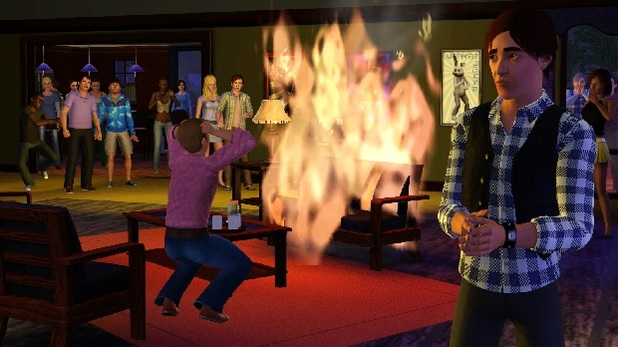
\includegraphics[scale=0.7]{SimsFire2}

~\\
We decided to create a separate collection of event-actions in order to allow an NPC to react in a different way than usual to an event. This makes sense considering an NPC's reaction to an alarm sounding would not be to grab him/herself a cup of coffee.
Since the algorithms discussed above are relatively generic, we can easily re-use these algorithms to create and weigh a graph of event-actions. 

~\\
Each event has the following properties 

\begin{enumerate}
\item A name and an Id.
\item Multiple variables concering the 'look and feel' of the event, including sounds and animations that should be played.
\item A duration.
\item An interest level minimum
\item An origin position.
\item A radius around this origin position.
\end{enumerate}

\newpage
Events are, in their most basic form, radiuses. When an NPC enters an event radius or happens to be there when an event is spawned, the NPC will instantly be prompted to react to the event.
Note that Events also have personality values of their own, which will be later used to calculate interest levels.

~\\
When an NPC comes close enough to an event, he/she will react to it in a way that matches the personality values of said NPC. This is accomplished in the following way:

~\\
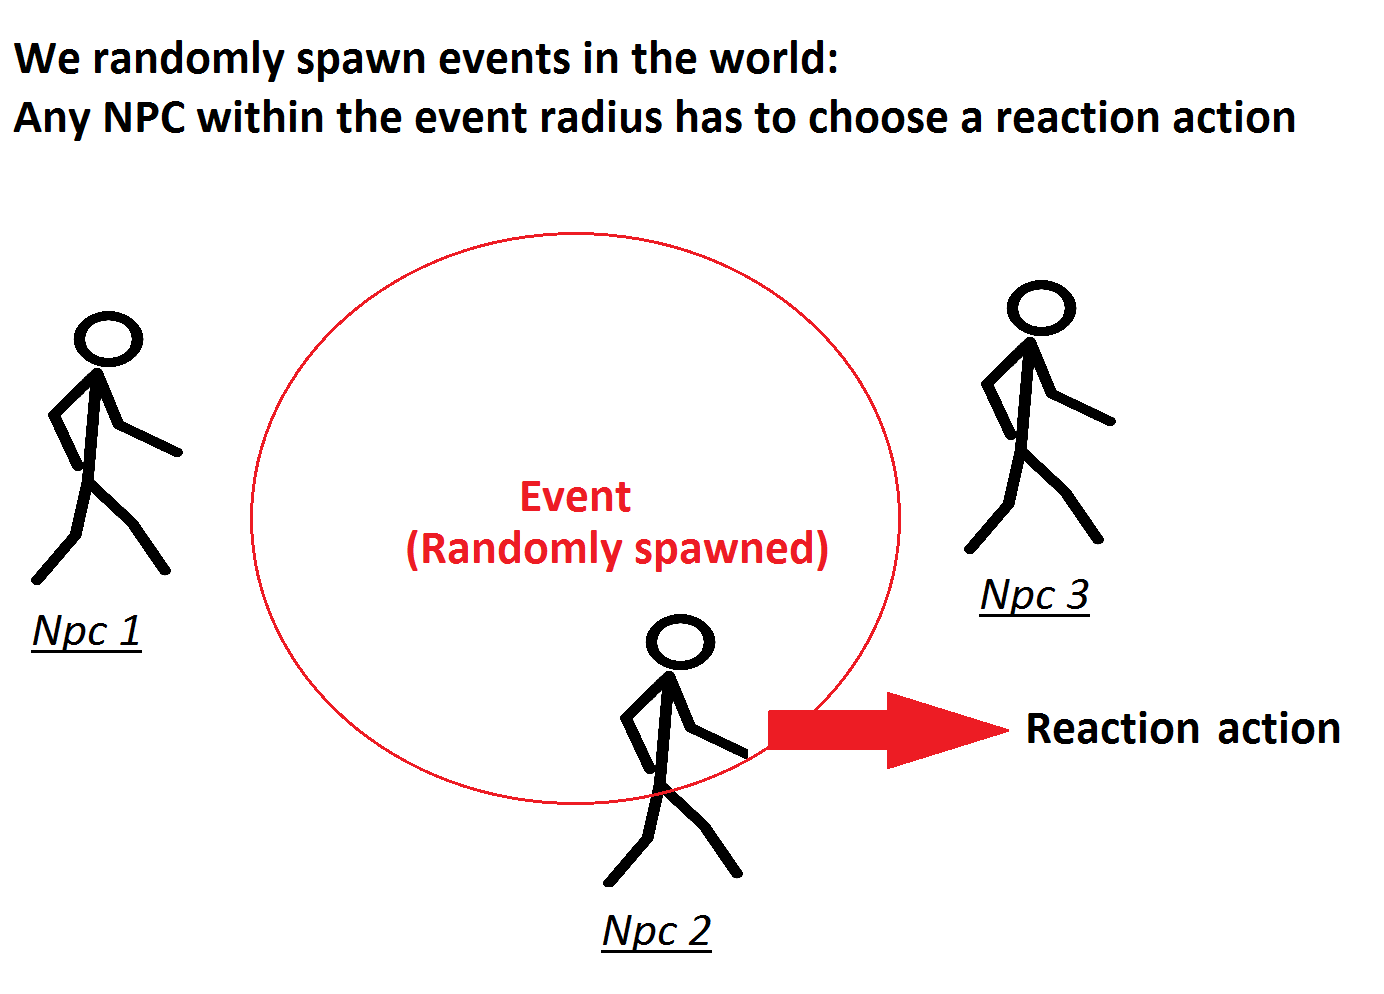
\includegraphics[scale=0.4]{Event}

~\\
In the Casanova code, we spawn a random event. This is done after a random time interval, making predicting when events will happen impossible for the player. Each NPC has a reference to the current active event (or, list, if there are multiple active events).

~\\
When an NPC enters the radius of an event, the algorithm that we discussed in the last chapter will change its' input nodes from normal action nodes, like getting coffee, to ' event action nodes'; actions that can only be performed when an NPC is near an active event.



\newpage
This transition is done instantly, so that the NPC does not casually finish drinking his coffee before reacting to the fainted individual next to him. Also, since event action nodes use exactly the same kind of XML variables as normal action nodes, the same algorithm can be used for both categories of actions. 

~\\
The duration property of the event determines, naturally, how long the event will be active.

~\\
An NPC is not obliged to react to an event. Just like in real life, not everything that happens around is us interesting enough for us to actively react to. Therefore, we compute an interest level for each NPC that enters an event radius, consisting of the result of the weighting algorithm on the personality values of the NPC and the personality, summed with 10 divided by the NPC's distance to the event and the amount of NPC's that are already reacting to the event.

~\\
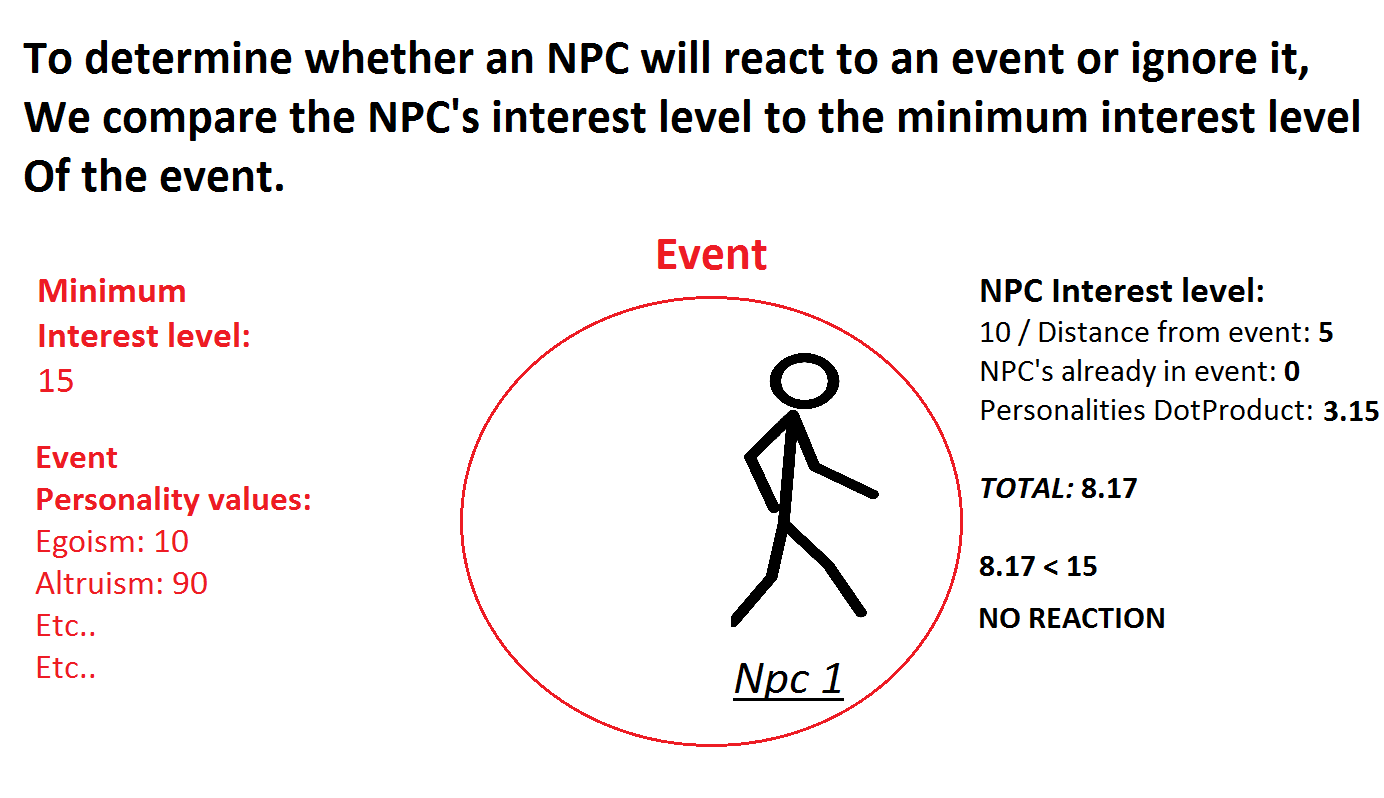
\includegraphics[scale=0.4]{InterestLevel}
~\\
 If the NPC's computed interest level is greater than or equal to the minimum interest level of the event, he/she will switch to the event reaction nodes instead of the normal action nodes, and react to the event. If not, the NPC will simply continue to perform normal actions, therefore ignoring the event.



\newpage
\section{Emotions}
We are currently researching how we can include emotion within our personality model, with the help of psychotherapist F. Steenbakkers, who is also a Phd candidate at the department for Clinical Psychology at Tilburg University. 

~\\
Ideally, we want the way in which NPC's decide what kind of behavior they will execute to be a close reflection of the way in which a real person does this; Personality models alone are not enough to accomplish this goal, so we hope that our cooperation with mr. Steenbakkers can lead us to a more realistic model for NPC behavior. 

~\\
Since we have, at the time of writing, only recently made contact with mr. Steenbakkers we do not have any major findings to report, but we will continue to work on integrating emotions and other psychological factors into our behavior model as this project goes along.

\newpage
\section{Player interaction}
In our original Architecture Document, we included a few examples of demo-games that might be created to demonstrate the virtual environment we will create. We decided to repeat them here with a few additions, since we believe they still are valuable demo-ideas (Despite the rest of the old Architecture Document being quite deprecated).


\subsection{Demo 1: Selecting certain NPC's}
We intend to demonstrate this project by creating a game, or several games, in which player NPC interaction and NPC personalities will be key concepts. The simplest and probably most usefull kind of demo would be to have the player walk around a group of NPC's and have the player identify the NPC who exhibits a certain personality trait the strongest. 

~\\
This would be quite easy to implement: The only addition that is needed is for us to randomly select a certain trait, then store which NPC has the highest score on that trait. Finally, some controls for the player need to be added and the demo is ready. 

~\\
Because we use an XML file to store the ranges a certain personality trait may exhibit for a given NPC population, we can easily create multiple XML files storing various personality ranges and feed them as input to the game whenever we choose, providing us with an easy way of showcasing different NPC populations.

\newpage
\subsection{Demo 2: Interrogation game}

~\\

\includegraphics[scale=0.7]{Interrogation}

~\\
A more complicated demonstration game would be to have the player interact one-on-one with an NPC within the context of an interrogation game. A possible way to implement this would be to have a certain NPC being suspected to have committed a certain crime, with the player tasked to ask questions about this crime and decide, based on the NPC's responses, body language and facial expression wether the NPC has committed the crime or not. 

~\\
This would require some extra additions to the vanilla concept, like generating random crimes, their circumstances and the NPC's degree of involvement in the crime. It might also require some more advanced facial animations in order to create a believable 'suspect'. If implemented well enough however, it might provide a very entertaining experience to the players. It might also provide data on wether the NPC's personalities can also shine through and be believable in a one-on-one situation.

\newpage
\subsection{Demo 3: Profiling challenge}

~\\
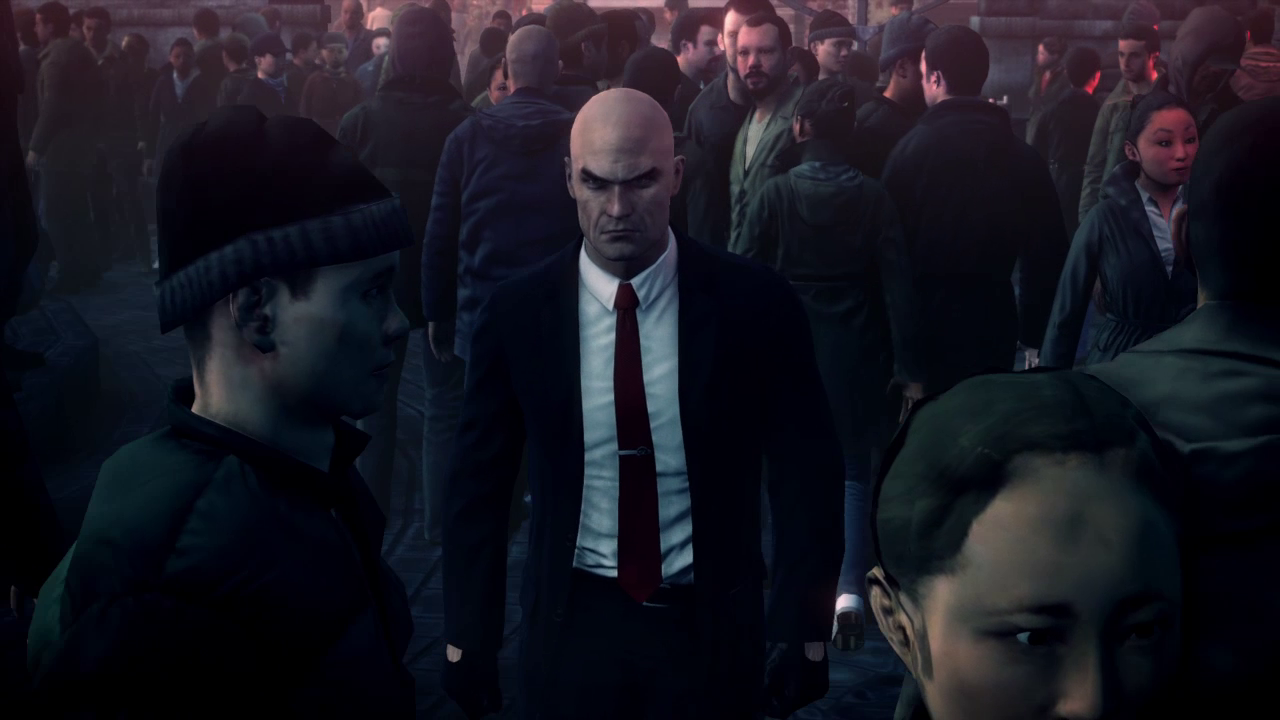
\includegraphics[scale=0.3]{Hitman}

~\\
Finally, we might expand on the first kind of demo by including more of a challenge factor. This could be done by giving the player a time limit to find an NPC with a certain trait-extreme or by giving a 'profiler' role to the player. 

~\\
This would involve the player having to pick out an NPC from a crowd who is most likely to be agressive or commit a crime, by carefully examining their behavior. This task can be made more challenging by giving the player only one chance: If they choose the wrong NPC, they lose instantly. 

~\\
This might require a more detailed personality model than our current one, which only measures 5 of the primary personality traits of humans. HEXACO, for example, includes factors like fear of physical pain, anxiety, patience etc. which could all be potential characteristics exhibited by criminals who are about to commit a crime.

~\\
Another variation on this 'spot the criminal'  idea could be having the character protect a VIP NPC; The player then has to pick out the non-VIP NPC most likely to harm the VIP, based on their behavior. 

~\\
All of these examples can provide an entertaining game with the ability to tell us how well the characters emulate real personalities; the amount of time and resources we will have available when we have established a good baseline for procedural avatar personality generation will influence which demoes we will and will not implement.



\newpage
\section{Other improvements}
The system as it currently stands has a lot of area for improvement. We still do not have any real art assets or character animations, making the NPC's look more like robots than persons. These cosmetic Personality and emotions are in our opinion of less importance than the bigger issue of NPC design. In a real person personality and emotions are, of course, not the only factors that influence that persons' behavior in a given situation. 


~\\
Upbringing, inherited traits, culture, social standing, group dynamic etc are all very important factors when trying to decipher why someone exhibits a certain kind of behavior.

~\\
Next up we will discuss the feasibility of including these factors within our simulation of human behavior, with the exception of upbringing:
including upbringing and inherited traits as factors within our virtual decision-making process would require two NPC's to combine their 'behavioral factors' in order to create a new NPC; while we consider this a very interesting subject, we believe it to be out of scope for this project. 

\newpage
\subsection{Adding NPC's from different cultures}
Introducing an NPC's culture into the mix could be a very valuable asset, if we represent cultural influence accurately enough. Having an accurate representation of the impact of culture on behavior could make this project into a training tool for international businesses, since unknowingly disrespecting a clients culture could have disastrous consequences.

~\\
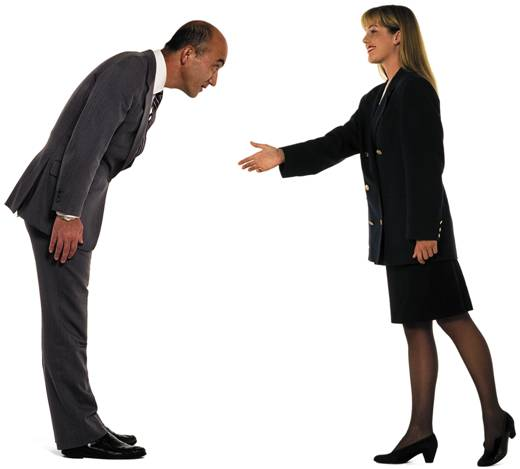
\includegraphics[scale=0.7]{Culture}

~\\
Important cultural differences lie mostly in areas such as personal space, appropriate ways of approaching a stranger etc. These kinds of interactions could be easily implemented by having NPC's react to the players' immediate presence in a way appropriate to their culture.


\newpage
\subsection{NPC groups}
Last but certainly not least, we will discuss the potential implementation of social standing and group dynamics within our project. Within psychology, groups are classified to be either a formal or informal group. 

~\\
Each of these categories can be further defined as either a command group, an interest group or a friendship group. Broadly speaking, formal command and interest groups are usually found within the work environment, while informal friend groups are more commonly found within clubs and friend groups. 

~\\

\includegraphics[scale=0.4]{SimsGroup}


~\\
Within the context of our project, we think informal friend groups are a good starting point.The other types of groups, especially the more formal types, always exist because of a higher, shared purpose which the NPC's in our system do not possess. 



\newpage
Informal friend groups however  (We will refer to them as IFG's for short) only exist because their members have shared interests or share certain personality traits. Especially the last kind of reason for an IFG to exist would be easy to implement within our system, since we already model our NPC's personalities. 

~\\
We could easily let NPC's with relatively proportionate personality values flock together one by one into a loose group. If we decide to dig deeper into the concept of group formation, we might also want to include the different stages of group formation that are known in psychology literature: %REFERENCE

~\\
A big challenge when implementing groups of NPC's is that of each individual NPC's autonomy level: How much does an individual decide for him/herself whilst being a member of a group, and how much does the NPC follow the leading group behavior? We will likely implement this with a chance function, in which the level of autonomy being given to each group member determines their chance of acting according to their own personality values, rather than follow majority group decisions. 

~\\
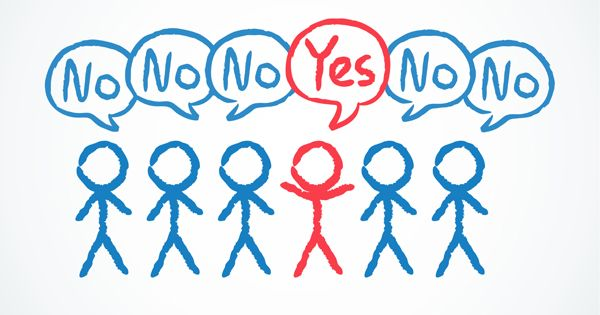
\includegraphics[scale=0.7]{PeerPressure}



~\\
This problem might be made easier if we limit NPC groups to NPC's with nearly identical personality values only: In this case, the homogenous personality values will ensure that most group-action decisions are made unanimously most of the time.

~\\
A further addition to this concept could be group stages: Distinct phases of the group's development, from the first contact of the group members until the disbanding of the group. Including these dynamic phases within our group concept would make the groups feel much more alive, rather than them simply being blobs of NPC's moving together.

~\\
\subsection{NPC to NPC interaction}
Finally, a big gap in our project as it currently stands is the absence of NPC to NPC interaction: We are still working on defining NPC to NPC interaction beyond NPC's merely not wanting to invade their personal spaces.

\newpage
\section{Planning}
We have made a preliminary, abstract planning for this project. Keep in mind that this planning will likely shift, and new tasks will certainly be added. For a more up-to-date version of this plan, please contact us to be granted access to our Google Agenda.

~\\
\begin{tabular}{|  l | l | l | }
  \hline			
  Task Name & Team Member & Deadline  \\ \hline
  Create basic event system & Steven & 7 October \\ \hline 
  Create initial cluster rendering test setup & Everyone & 23 October \\ \hline 
  Implement Yossi / Max Weight Matching Algorithm & Cees-Jan & 23 October \\ \hline
  Buy  art assets & Everyone & 26 October \\ \hline 
  Expand event system & Robert and Steven & 28 October \\ \hline  
  Connect NPC emotions to personality & Everyone & 4 November \\ \hline
  Create different game-modes & Robert and Cees-Jan & 11 November \\ \hline
  Create improved cluster rendering implementation & Steven & 25 November \\ \hline  
  Present the final product, deliver documentation & Everyone & End of december \\ \hline
\end{tabular}
\end{document}